\chapter{Operações Unitárias II}
\section{Relembrando}
\subsection{Fenômenos de Transporte II}
Tendo dois diferentes materiais em temperaturas diferentes, um com uma temperatura maior, outra
menor é observado um fluxo de calor em saindo do de maior temperatura para o de menor temperatura. A
diferença de temperatura, ou seja, a formação de um gradiente de temperatura é a força motriz para o
acontecimento da transferência de calor. \par

Na literatura, os três tipos distintos da transmissão de calor são a condução, a convecção e a
radiação. A condução e a radiação podem ser caracterizadas por um gradiente de temperatura, enquanto
a convecção é a transmissão de energia de regiões com maior temperatura para aquelas de menor
temperatura. Esses três tipos de transmissão de calor podem ocorrer simultaneamente, ou podem
dominar um sobre o outro, dependendo das condições do sistema. \par
% Fim Introdução
%────────────────────────────────────────────────────────────────────────────────────────────────────────────────────────────────────────────────────

\subsection{Condução}
Por definção esse mecanismo necessita de contato físico entre os meios, onde por meio desse contato,
o calor fluirá do meio com maior temperatura para o meio com menor temperatura. Essa fluidização,
ocorre por meio de vibrações atômicas, onde os átomos transferem energia para os outros átomos. Esse
meio é o único que pode ocorrer em sólidos opacos. \par

A equação que rege esse fenômeno é a \emph{Lei de Fourier}:
\begin{equation}\label{eq:fourier}
    q = - KA \frac{\mathrm{d}T}{\mathrm{d}x} 
\end{equation}
Onde $q$ é a taxa de transferência de calor, $K$ é a condutividade térmica, $A$ é a área de
transferência de calor e $\frac{\mathrm{d}T}{\mathrm{d}x}$ é o gradiente de temperatura. \par
% Fim Condução
%────────────────────────────────────────────────────────────────────────────────────────────────────────────────────────────────────────────────────
\subsection{Radiação}
Esse mecanismo de transferência de calor ocorre por meio de ondas eletromagnéticas, que podem ser
caracterizadas por sua frequência e comprimento de onda. A radiação térmica é emitida por todos os
corpos com temperatura acima do zero absoluto. Por ser dependente de ondas eletromagnéticas, ela é a
única que não precisa de máteria para ocorrer, podendo ser transmitida no vácuo. \par

A radiação viaja na velocidade da luz, e é modelada por meio da equação de Stefan-Boltzmann:
\begin{equation}\label{eq:stefan-boltzmann}
    q = \sigma A T^4
\end{equation}
Onde $q$ é a taxa de transferência de calor, $\sigma$ é a constante de Stefan-Boltzmann, $A$ é a
área de transferência de calor e $T$ é a temperatura absoluta. \par

Caso o corpo esteja irradiando para outro corpo, a equação de Stefan-Boltzmann é modificada para
\begin{equation}\label{eq:stefan-boltzmann2}
    q = \sigma A (T_1^4 - T_2^4)
\end{equation}
Onde $q$ é a taxa de transferência de calor, $\sigma$ é a constante de Stefan-Boltzmann, $A$ é a
área de transferência de calor, $T_1$ é a temperatura absoluta do corpo que está irradiando e $T_2$
é a temperatura absoluta do corpo que está recebendo a radiação. \par
% Fim Radiação
%────────────────────────────────────────────────────────────────────────────────────────────────────────────────────────────────────────────────────
\subsection{Convecção}
Esse mecanismo de transferência de calor ocorre por meio de um fluido, que pode ser um líquido ou
um gás. Esse fluido é aquecido, e por meio de sua movimentação, o calor é transferido para outro
corpo. \par

A equação que rege esse fenômeno é a \emph{Lei de Newton}:
\begin{equation}\label{eq:lei_newton}
    q = h A (T_1 - T_\infty )
\end{equation}
Onde $q$ é a taxa de transferência de calor, $h$ é o coeficiente de transferência de calor, $A$ é a
área de transferência de calor, $T_s$ é a temperatura absoluta do corpo e $T_\infty $ é a temperatura
absoluta do fluído. \par

O coeficiente de transferência de calor é uma propriedade do fluído, e depende de sua velocidade,
viscosidade, densidade, condutividade térmica e outras propriedades. \par

\subsubsection{Convecção Natural}
Esse tipo de convecção ocorre por meio de diferenças de densidade, ou seja, por meio de diferenças
de temperatura. Ela ocorre sem interferência de forças externas, como bombas ou ventiladores, sendo
geradas pela diferença de densidade entre o fluído aquecido e o fluído resfriado. \par

\subsubsection{Convecção Forçada}
Se deve a interferência de forças externas, como bombas ou ventiladores, que movimentam o fluído
aquecido. Independe de forças de densidade e flotação. \par
% Fim Convecção
%Fim do Relembrando
%────────────────────────────────────────────────────────────────────────────────────────────────────────────────────────────────────────────────────
\section{Propriedades Termofísicas}
Durante o estudo de transferência de calor, muitas vezes tinhamos propriedades termofísicas
constantes, com valores uniformes. Porém, na prática, essas propriedades são dependentes de diversos
fatores de formas que em muitos casos não podem ser consideradas constantes. \par

O fato de variarem, muitas vezes com a temperatura, ou outros, são limitantes para resolução do
problema, gerando erros de cálculos e faltas de exatidão. Essas propriedades são muito importantes e
em processos, como os que possuem alimentos, o erro ou a falta de precisão nesses cálculos podem
causar mudanças drásticas no sabor e valor nutricional do produto final. \par

As propriedades termofísicas mais importantes são a condutividade térmica, calor específico,
difusividade térmica e densidade. \par
% Começo de Propriedades Termofísicas
\subsection{Condutividade Térmica}
A condutividade térmica é uma propriedade que indica a capacidade de um material de conduzir calor.
Os métodos de medição podem variar desde medições diretas, tabelas pré-calculadas, correlações e
valores estimados. \par

Algumas equações empíricas são apresentadas abaixo, cada uma com sua aplicação:
\begin{enumerate}
    \item {Equação de Sweat, para carnes e peixes:
        \begin{equation}\label{eq:sweat}
            k  = 0.08 + 0.52 X_{w}
        \end{equation}}
    \item {Equação de Kolarov e Gromov, para sucos e frutas:
        \begin{equation}\label{eq:kolarov}
            k  = 0.14 + 0.42 X_{w}
        \end{equation}}
    \item {Equação de Choi e Okos, para gerais:
        \begin{equation}\label{eq:choi}
            k  = 0.61 X_{w} + 0.20 X_{p} + 0.205 X_{c} + 0.175X_{f} + 0.135X_{a} 
        \end{equation}
        Onde $X_{w}$ é a fração de água, $X_{p}$ é a fração de proteína, $X_{c}$ é a fração de
        carboidrato, $X_{f}$ é a fração de gordura e $X_{a}$ é a fração de cinzas.}
\end{enumerate}
Já para acima do ponto do congelamento nossas equações ficam
\begin{enumerate}
    \item {equação de Sweat:
        \begin{equation}\label{eq:sweat2}
            k  = 0.148 + 0.493X_{w} \
        \end{equation}
        Válida para frutas e vegetais, com exceção de maçã in natura.}
        \item {equação de de Choi e Okos:
            \begin{equation}\label{eq:choi2}
                k = \sum_{i} \left( K_{i}  X_i^{V}  \right)
            \end{equation}
            Ela é válida quando se conhece a composição dos alimentos. A fração volumétrica do
            componente \(i\) é dada por:
            \begin{equation}\label{eq:fracao_volumetrica}
                X_i^{V} = (X_i^{m}/\rho_i) / \sum_{i} (X_i^{m}/\rho_i)
            \end{equation}
            Onde \(X_i^{m}\) é a fração mássica do componente \(i\) e \(\rho_i\) é a densidade do
            componente \(i\), \(K_{i} \) é a condutividade térmica do componente \(i\), \(K\) é a
            condutividade térmica e \(X_{w} \) é  a fração de água.}
\end{enumerate}
Para situações abaixo do ponto de congelamento temos
\begin{enumerate}
    \item {Equação de Jowitt:
        \begin{equation}\label{eq:jowitt}
            k = 2.44X_{w} + \left( 1 - X_{w}  \right) 0.26
        \end{equation}}
        \item {Equação de Fikiin
            \begin{equation}\label{eq:fikiin}
                k = 1.745X_{w} \left( 1 - \frac{T_{f} }{T} \right) + 0.233
            \end{equation}
            Onde \(T_{f} \) é a temperatura de início de congelamento e \(T\) é a temperatura da amostra}
\end{enumerate}  
% Fim de Condutividade Térmica
\subsubsection{Exexmplo 1}
Determinar a condutividade térmica de uma carne com 70\% de água a \(-2 \degree C\)
\paragraph{Solução}
Aplicando a fórmula de Sweat, enunciada em \ref{eq: sweat}, temos:
\begin{align*}
    k &= 0.148 + 0.493 \cdot  0.7\\ 
    &= 0.4931 \; \frac{W}{m \cdot K}
\end{align*}
% Fim Exemplo 1
\subsubsection{Exemplo 2}
Determinar a condutividade térmica do suco de laranja a \(3 \degree C\) com aproximadamente 89\% de
água.
\paragraph{Solução}
Aplicando a equação de Kolarov e Gromov, enunciada em \ref{eq:kolarov}, temos:
\begin{align*}
    k &= 0.14 + 0.42 \cdot  0.89\\
    &= 0.5138 \; \frac{W}{m \cdot K}
\end{align*}
% Fim Exemplo 2
% Fim exemplos 
Uma outra forma de conseguirmos calcular a condutividade térmica é por meio de medidas
experimentais, onde por meio de uma célula especificadamente projetada para isso, por medição da
amostra e de alguns outros conehcimento prévios, consegue-se calcular o valor da condutividade, que
é dado pela equação abaixo:

\begin{equation}\label{eq:medida_experimental}
    k = \dot{q} \frac{\log \frac{R_2}{R_1}}{2\pi L\left( T_1 - T_2 \right) }
\end{equation}
Onde \(\dot{q}\) é o fluxo de calor, \(L\) é comprimento do cilindro de raio \(r\)
% Fim da Condutividade térmica
%────────────────────────────────────────────────────────────────────────────────────────────────────────────────────────────────────────────────────
\subsection{Calor Específico}
O calor específico é uma propriedade que indica a quantidade de calor necessária para elevar a
amostra em uma unidade de temperatura. Ela pode ser definida como a variação da entalpia \(H\) pela
temperatura, ou seja:
\begin{equation}\label{eq:calor_especifico_derivada }
    C_{p}  = \frac{dH}{dT}
\end{equation}
Os métodos de obtenção do calor específico incluem, medição direta, tabelas ou gráficos, nomogramas,
correlações empíricas e valores semelhantes. \par

Algumas correlações empíricas para o calor específico, acima do ponto de congelamento, são:
\begin{enumerate}
    \item {Equação de Siebel:
        \begin{equation}\label{eq:siebel}
            C_{p}  = 0.837 + 3.349X_{w} 
        \end{equation}}
    \item {Equação de Charm:
        \begin{equation}\label{eq:charm}
            C_{p}  = 2.309X_{G} + 1.256X_{s} + 4.186X_{w}
        \end{equation}
        Onde \(X_G\) é a fração mássica de gorudra, \(X_s\) é a fração mássica de sólido e \(X_w\) é a
        fração mássica de água}
        \item {Equação de Choi e Okos:
                \begin{equation}
                    C_{p}  = \sum_{i} \left( C_{p_{i}} X_i^{m}  \right)  
                \end{equation}
                Onde \(C_{p_{i}}\) é o calor específico do componente \(i\) e \(X_i^{m}\) é a fração
                mássica do componente \(i\)}
\end{enumerate}
Abaixo do ponto de congelamento temos:
\begin{enumerate}
    \item {Equação de Miles:
        \begin{equation}\label{eq:miles}
            C_{p}  = 1256X_{w} + 837\
        \end{equation}}
    \item {Equação de Jowitt:
        \begin{equation}\label{eq:jowitt_cp}
            C_{p}  = \left( 2093 \left( \frac{T_{f} }{T} \right) + 837 \right) X_{w} + 1382
        \end{equation}
        Onde \(T_{f} \) é a temperatura de início de congelamento e \(T\) é a temperatura da
        amostra}
\end{enumerate}
\subsubsection{Exemplo 1}
Determinar o calor específico de carne de frango fresco e congelado a \(-2.8 \degree C\). A carne de
frango possui aproximadamente 74\% de água com início de congelamento a \(2.8 \degree C\)
\paragraph{Solução}
Para o frango fresco, vamos utilizar a equação de Siebel, enunciada em \ref{eq:siebel}, temos:
\begin{align*}
    C_{p} &= 0.837 + 3.349 \cdot  0.74\\
    &= 3.31526 \; \frac{kJ}{kg \cdot K}
\end{align*}
Para o frango congelado, vamos utilizar a equação de Jowitt, enunciada em \ref{eq:jowitt_cp}, temos:
\begin{align*}
    C_{p} &= \left( 2093 \left( \frac{2.8}{-2.8} \right) + 837 \right) 0.74 + 1382\\
    &= 452.56 \; \frac{J}{kg \cdot K}
\end{align*}
% Fim Exemplo 1
% Fim do Calor específico
\subsection{Difusividade Térmica}
Essa propriedade se relaciona com a velocidade a qual o calor consegue espalhar pelo material. Ela
pode ser definida como:
\begin{equation}\label{eq:difusividade_termica}
    \alpha = \frac{k}{\rho C_{p} }
\end{equation}
Com unidades em \(\frac{m^2}{s}\). Sua determinação depende de outras constantes também, sendo
bastante demorada e requerendo considerável trabalho experimental. \par

Essa propriedade é de fundamental importância, principalmente quando falamos de regime transiente,
já que ela ajuda a estabelecer a rapidez com que o calor se propaga no material e ajuda a estabeler
o grau de dependência de tempo da temperatura. \par

Ela pode ser determinada, através de experimentos, achada por meio de tabelas, correlações e valores
semelhantes. \par

\subsubsection{Exemplo 1}
Determinar a função matemática que represent difusividade térmica da água em função da temperatura.
Os dados são apresentados abaixo:
\begin{table}[H]
\centering
\begin{tabular}{c|c}
\toprule
T \((\degree C)\)  &  \(\alpha \; \left( \frac{m^{2}}{s \cdot 10^{7} } \right) \)  \\
 \midrule
 0&1.31   \\
  4&1.34 \\
  10&1.38   \\
  15.6&1.41   \\
  21.1&1.44   \\
  26.7&1.46   \\
  32.2&1.49   \\
  37.8&1.51   \\
    43.3&1.54   \\
    48.9&1.55   \\
    54.4&1.57   \\
    60&1.59   \\
    65.6&1.61   \\
    71.1&1.62   \\
    76.7&1.64   \\
    82.2&1.65   \\
    87.8&1.66   \\
    93.3&1.67   \\
\bottomrule
\end{tabular}
\caption{Dados Coletados Experimentalmente}
\label{tab:tabela_dif_ex1}
\end{table}
\paragraph{Solução}
Para determinar a função matemática que representa a difusividade térmica da água em função da
temperatura, vamos primeiros visualizar os dados em um gráfico, para termos uma ideia de qual modelo
ela poderia se ajustar. Pelo seguinte código no python conseguimos visualizar os dados:  
\begin{minted}{python}
    import matplotlib.pyplot as plt
    import numpy as np
    import scienceplots
    plt.style.use(['science', 'notebook'])


    T = np.array([0, 4, 10, 15.6, 21.1, 26.7, 32.2, 37.8, 43.3,
        48.9, 54.4, 60, 65.6, 71.1, 76.7, 82.2, 87.8, 93.3])
    alpha = np.array([1.31, 1.34, 1.38, 1.41, 1.44, 1.46, 1.49, 1.51,
        1.54, 1.55, 1.57, 1.59, 1.61, 1.62, 1.64, 1.65, 1.66, 1.67])

    plt.plot(T, alpha, 'o')
    plt.xlabel(r'Temperatura ($\degree C)$')
    plt.ylabel(r'Difusividade Térmica $ \alpha \; (\frac{{m^2}}{{s}})$')
    plt.grid()
    plt.show()
\end{minted}
\begin{figure}[H]
    \centering
    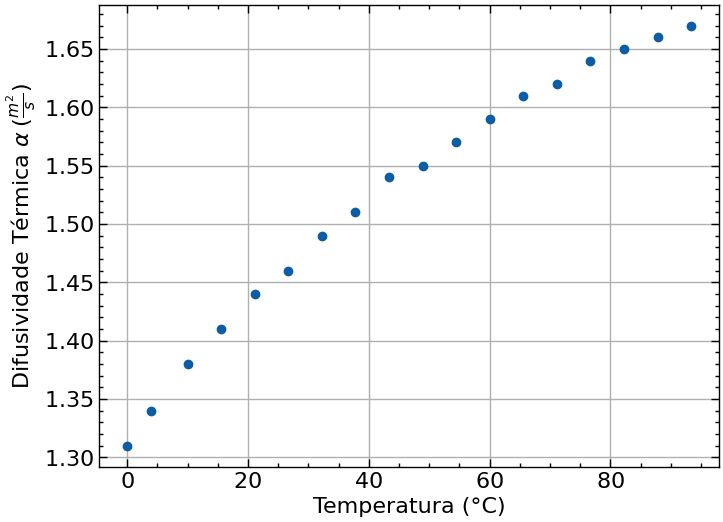
\includegraphics[width=0.8\textwidth]{difusividade_ex1}
    \caption{Gráfico dos dados experimentais}
    \label{fig:grafico_dif_ex1}
\end{figure}
Ao visualizar o gráfico, podemos perceber que os dados parecem estar em uma parábola, então vamos
tentar ajustar uma parábola aos dados. Para isso, vamos utilizar o método dos mínimos quadrados,
com o seguinte código:
\begin{minted}{python}
    import numpy as np
    from scipy.optimize import curve_fit

    T = np.array([0, 4, 10, 15.6, 21.1, 26.7, 32.2, 37.8, 43.3,
        48.9, 54.4, 60, 65.6, 71.1, 76.7, 82.2, 87.8, 93.3])
    alpha = np.array([1.31, 1.34, 1.38, 1.41, 1.44, 1.46, 1.49, 1.51,
        1.54, 1.55, 1.57, 1.59, 1.61, 1.62, 1.64, 1.65, 1.66, 1.67])

    def func(T, a, b, c):
        return a * T**2 + b * T + c

    popt, pcov = curve_fit(func, T, alpha)
    print(popt)

    plt.plot(T, alpha, 'o')
    plt.plot(T, func(T, *popt), 'r-')
    plt.xlabel(r'Temperatura ($\degree C)$')
    plt.ylabel(r'Difusividade Térmica $ \alpha \; (\frac{{m^2}}{{s}})$')
    plt.grid()
    plt.show()
\end{minted}
Onde a função \texttt{func} é a função que representa a parábola, e \texttt{popt} é um vetor que
contém os coeficientes da parábola. O resultado obtido foi:
\begin{minted}{python}
    [-2.48992854e-05  6.08503806e-03  1.31723970e+00]
\end{minted}
Note a falta do \(10^7\), nos valores. O correto é dividir todos os coeficientes por esse fator de
escala. O gráfico obtido foi:
\begin{figure}[H]
    \centering
    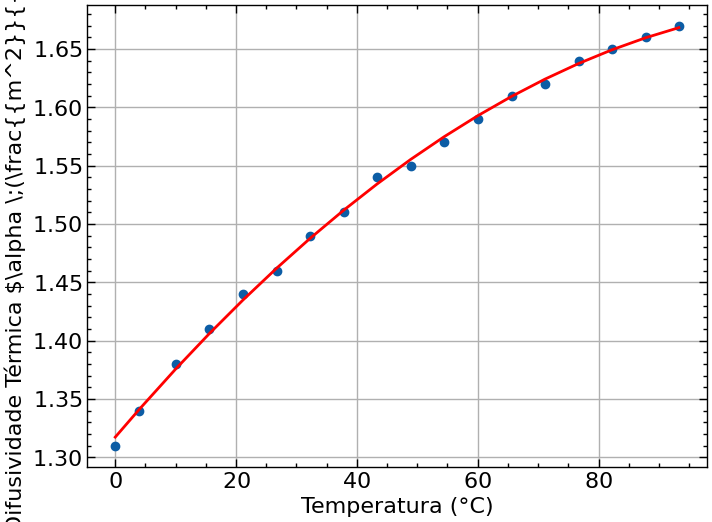
\includegraphics[width=0.8\textwidth]{difusividade_ex1_ajustada}
    \caption{Gráfico dos dados experimentais ajustados}
    \label{fig:grafico_dif_ex1_ajustado}
\end{figure}
Portanto, a função que representa a difusividade térmica da água em função da temperatura é:
\begin{equation}
    \alpha = 1.32 \cdot 10^{-7} + 6.11 \cdot 10^{-10} T - 2.48 \cdot 10^{-12} T^{2}
\end{equation}
\subsection{Densidade}
A densidade é uma propriedade física que relaciona a massa de um material com o seu volume. A
densidade é uma propriedade intensiva, ou seja, não depende da quantidade de matéria presente.
Ela é definida como:
\begin{equation}
    \rho = \frac{m}{V}
\end{equation}
Os métodos de determinação são experimentais, por tabelas ou gráficos, por equações empíricas ou
valores semelhantes. A equação empírica mais utilizada é a equação de Choi e Okos:
\begin{equation}
    \rho = \frac{1}{\sum_{i} \left( X_i^{m}/\rho _{i}   \right) }
\end{equation}
Onde \(X_i\) é a fração mássica do componente \(i\), \(\rho _{i}\) é a densidade do componente \(i\).
\section{Introdução a Condutores de calor}
Trocadores de calor são equipamentos que tem como função transferir calor de um fluido para outro,
seja para resfriamento, seja para aquecimento. Eles são amplamente utilizados em processos
industriais, como em refinarias, usinas de açúcar e álcool, usinas nucleares, etc. Eles podem ser
classificados de acordo com a direção do fluxo dos fluidos, de acordo com o número de fluidos
envolvidos, etc. \par

O ponto de referência que temos é o fluido principal, onde é ele que vamos ter que prestar mais
atenção. Vamos estudar 3 tipos de trocadores de calor, principalmente para seu dimensionamento, que
serão o trocador tubo duplo, o trocador casco e tubos e o trocador de placas. \par

\section{Trocador Tubo Duplo}
Composto por 2 tubos concêntricos, geralmente com 2 trechos retos, com conexões que permitem o
movimento do fluido de uma seção para outra. O conjunto no todo em forma de U é denominado de
grampo. Na parte curva do trocado de calor, não há troca de calor entre os fluídos, sendo
desconsideradas na análise. \par

O fluidos podem operar em contracorrente ou em corrente paralela. Onde em contracorrente é mais
utilizado por gerar trocadores com áreas menores. As vantagens desses trocadores incluem sua
facilidade de construção e montagem, facilidade de ampliação, manutenção, etc. \par

Os tubos concêntricos conduzem duas correntes, cada um com um coeficiente convectivo diferente e com
temperaturas de entrada e saída distintas. Geralmente, a fim de estabelecer a diferença de
temperatura entre o fluido quente \(T\) e o fluido frio \(t\) é necessário levar em conta todas as
resistências entre a temperaturas. \par

Nesse tipo de trocador de calor as resistências encontradas são as da resistências do fluido,
resistência da parede do tubo e a resistência do fluido anelar, ou seja:
\begin{equation}\label{eq:resistencia_tubo_duplo_geral }
    \frac{1}{U} = \sum_{i} R_{i}  =\frac{1}{h_1} + \frac{L}{K} + \frac{1}{h_0}
\end{equation}
Onde \(U\) é o coeficiente global de transferência de calor. Para um tubo com parede grossa, nossa
equação fica
\begin{equation}\label{eq:resistencia_tubo_duplo_parede_grossa_externo }
    \frac{1}{U_{ext}} = \frac{1}{h_{int}} + \frac{D_{ext} }{D_{int}} + \frac{1}{2} \frac{D_{ext} }{K} \ln \frac{D_{ext} }{D_{int}} + \frac{1}{h_{ext}}
\end{equation}
Ou, em relação ao interno:
\begin{equation}\label{eq:resistencia_tubo_duplo_parede_grossa_interno }
    \frac{1}{U_{int}} = \frac{1}{h_{int}} + \frac{1}{2} \frac{D_{int}}{K} \ln \frac{D_{ext} }{D_{int}} + \frac{1}{h_{ext}}\frac{D_{int }}{D_{ext} }
\end{equation}
A transferência de calor por combinação da condução e convecção pode ser dada em relação ao
coeficiente global de transferência de calor:  
\begin{equation}\label{troca_de_calor_U}
    q = UA \Delta T
\end{equation}
Onde \(A\) é a área de troca de calor, \(\Delta T\) é a diferença de temperatura entre as correntes
para toda superfície \(A\). \par

O perfil de temperatura se difere quando falamos de correntes opostas ou em correntes paralelas.
Pelo gráfico abaixo podemos ver a diferença entre os dois perfis:
\begin{figure}[H]
    \centering
    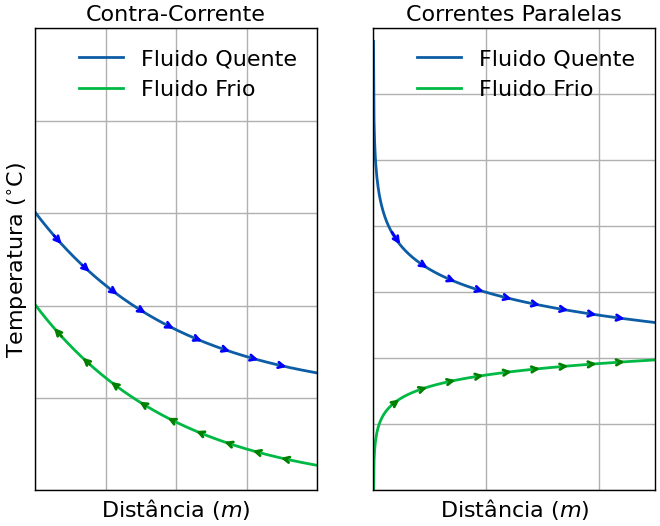
\includegraphics[width=0.8\textwidth]{diferenca_correntes}
    \caption{Diferença entre correntes paralelas e contracorrentes}
    \label{fig:diferenca_correntes}
\end{figure}
\subsubsection{Fatores de Incrustação}
Os fatores de incrustação são fatores que levam em conta a sujeira que pode se acumular na parede
dos tubos, diminuindo a área de troca de calor. Ocorre um aumento da resistência térmica, diminuindo
o desempenho térmico do trocador. \par

A formação de incrustações pode ser causado por diversos fatores, como a corrosão, sedimentação,
cristalização, dentre outros, todos que dependem do tipo de fluido e as características de
escoamento. \par

Incrustações na parte interna e externa do nosso tubo causará um acréscimo de duas resistências, que
deverão ser adicionadas na equação \ref{eq:resistencia_tubo_duplo_geral}, equação que passará a ser
chamada de equação limpa. Nossa equação ficará:
\begin{equation}\label{eq:resistencia_tubo_duplo_incrustado}
    \frac{1}{U_{d}} = \frac{1}{h_{int}} + \frac{1}{h_{ext}} + R_{di} + R_{de} 
\end{equation}
%────────────────────────────────────────────────────────────────────────────────────────────────────────────────────────────────────────────────────
\subsection{Exemplo}
Deseja-se aquecer \(4000 \;\frac{kg}{h}\) de suco de laranja de 26 para 42 \(^{\circ}C\) utilizando  
\(5000 \; \frac{kg}{h}\) de água quente à \(72 \; \degree C\). Um fator de incrustação de \(0.0001
\; h m^{2} \degree \frac{C}{kcal}\) pode ser disponível para cada corrente. Além disso, a pressão
permitida para cada corrente é de \(1 \; \frac{kgf}{cm^{2}}\). Dispõe-se de um certo número de tubos
anulares de 6 metros com tubos IPS de diâmetro nominal de \(2^{\prime \prime} \; x \;
1^{\frac{1}{4}^{\prime \prime} } \). Quantos metros de tubos são necessários? \par

\subsubsection{Primeira Solução}
Para a primeira forma de solução, vamos utilizar o método de Kern. Primeiro fazer o balanço de
energia
\begin{align}
    \dot{M}C_{p} \Delta T &= \dot{m}  c_p \Delta t \\
    T_2 = T_1 - \frac{\dot{M} C_p \Delta T}{\dot{m}c_{p}}
\end{align}
Vamos precisar das propriedades termofísicas na temperatura média, que será
\begin{align}
    \overline{T}_{suco} = \frac{T_1 + T_2}{2} = \frac{26 + 42}{2} = 34 \; ^{\circ}C \\
    \overline{T}_{\acute{a}gua} = \frac{T_1 + T_2}{2} = \frac{72 + 28}{2} = 50 \; ^{\circ}C
\end{align}
Onde o \(28\degree C\) foi um chute aleatório. De acordo com a apostila, o suco de laranja \(11
\degree \) Brix possui as seguintes propriedades:
\begin{align}
    C_{p} &= 3.89 \; \frac{kJ}{kg \; ^{\circ}C} \\
    K &= 0.554 \; \frac{W}{m \; ^{\circ}K}\\
    \rho &= 1.043 \; \frac{kg}{m^{3}} \\  
\end{align}
Sendo ele um fluído não newtoniano, temos também que
\begin{align}
    k &= 0.05 \; Pa.s^{n} \\
    n &= 0.8
\end{align}
Para a água, temos
\begin{align}
    C_{p} &= 4180.7 \; \frac{kJ}{kg \; ^{\circ}C} \\
    K &= 0.64 \; \frac{W}{m \; ^{\circ}C}\\
    \rho &= 998.037 \; \frac{kg}{m^{3}} \\
    \mu &= 0.546 \cdot 10^{-3} \; Pa.s
\end{align}
Com isso, conseguimos a temperatura final da água:
\begin{align}
    T_2 &= T_1 + \frac{\dot{M} C_p \Delta T}{\dot{m}c_{p}} \\
    T_2 &= 72 - \frac{4000 \cdot 3890 \cdot (42 - 26)}{5000 \cdot 4180.7} \\
    T_2 &= 60 \; ^{\circ}C
\end{align}
Agora, vamos recalculas as propriedades da água na temperatura média:
\begin{align}
    \overline{T}_{\acute{a}gua} &= \frac{T_1 + T_2}{2} = \frac{72 + 60}{2} = 66 \; ^{\circ}C 
\end{align}
Como as propriedades não se alteraram muito, esse processo de iteração pode ser feito apenas uma vez
sendo assim, satisfatório. \par

Vamos agora calcular a \(MLDT\). O trocador de calor é de correntes opostas, então
\begin{align}
    MLDT &= \frac{\Delta T_2 - \Delta T_1}{\ln \frac{\Delta T_2}{\Delta T_1}} \\  
    &= \frac{4}{\ln \frac{34}{30}}\\
    &= 31.96 \; ^{\circ}C
\end{align}
Agora, vamos calcular o número de Reynolds para o fluido quente, no ânulo:
\begin{align}
    Re &= \frac{\rho \upsilon D_{eq} }{\mu }
\end{align}
Onde os diâmetros dos tubos, ao quadrado, são
\begin{align}
    D_{int}^{2^{\prime\prime}} = 0.0545 \; m^{2} \\
    D_{ext}^{1 \frac{1}{4}^{\prime \prime}} = 0.0421 \; m^{2}\\
    D_{ext}^{2^{\prime\prime}} = 0.0603 \; m^{2}  
\end{align}
A velocidade pode ser dada por
\begin{align}
    \upsilon &= \frac{\dot{m}}{\rho A} \\
    &= \frac{5000 \cdot 1/3600}{\pi/4 \left[ \left( 0.0525 \right) ^{2} - \left( 0.0421 \right) ^{2}  \right] 998.037}\\
    &= 1.8 \frac{m}{s}
\end{align}
O número de Reynolds é então
\begin{align}
    Re &= \frac{998.037 \cdot 1.8 \cdot 0.0104}{0.546 \cdot 10^{-3}}\\
       & = 34218
\end{align}
O que caracteriza um regime turbulento. \par

Agora, vamos calcular o \(h_{parede,\acute{a}gua}\). Para isso, vamos calcular o número de Nusselt
\begin{align}
    Pr &= \frac{C_p \mu}{K} = (4180 \cdot 0.546 \cdot 10^{-3})/0.64 = 3.57\\
    Nu &= \frac{hD}{K} = 0.023 Re^{0.8} Pr^{0.33} \left( \frac{\mu_b}{\mu _{b} } \right)  \\
    &= 0.023 \cdot 34218^{0.8} \cdot 3.57^{0.33} \left( \frac{0.546 \cdot 10^{-3}}{0.546 \cdot 10^{-3}} \right)  \\
    &= 149\\
    149 &= \frac{hD}{K} \\
    h &= \frac{149 \cdot 0.64}{0.0104} = 9169.2 \; \frac{W}{m^{2} \; ^{\circ}C}
\end{align}
Similarmente, vamos fazer o mesmo para o suco. Primeiro o número de Reynolds
\begin{align}
    Re &= \frac{\rho \upsilon ^{2-n} D^{n} }{8^{n-1} K} \left( \frac{4n}{3n + 1} \right)^{n} \\
\end{align}
Com diâmetros e velocidades
\begin{align}
    D_{int}^{1 \frac{1}{4}^{\prime \prime}} &= 0.035 \;\\
    D_{ext}^{1 \frac{1}{4}^{\prime \prime}} &= 0.0421 \;\\
    \upsilon &= \frac{\dot{m}}{\rho A} \\
    &= \frac{4000 \frac{1}{3600}}{\frac{\pi}{4}\left( 0.035 \right)^{2} 1043 }\\
    &= 1.1 \frac{m}{s}
\end{align}
Por fim, como já colocado, \(n = 0.8\) e \(K = 0.05 \; Pa.s^{n}\), temos
\begin{align}
    Re &= \frac{1043 \cdot 1.1^{2-0.8} \cdot 0.035^{0.8} }{8^{0.8-1} \cdot 0.05} \left( \frac{4 \cdot 0.8}{3 \cdot 0.8 + 1} \right)^{0.8} \\
    &= 2310.9
\end{align}
Sendo considerado regime laminar. Agora, vamos calcular o número de Nusselt, para depois calcularmos
o \(h_{parede_suco}\)
\begin{align}
    Nu &= \frac{hD}{K} = 1.75 \delta ^{\frac{1}{3}} G_{z}^{\frac{1}{3}} \left( \frac{\rho _{b} }{\rho _{p} } \right) \\
    \delta &= \frac{3n+1}{4n} = (3 \cdot 0.8 + 1)/(4 \cdot 0.8) = 1.06 \\
\end{align}
O \(G_{z} \) é o número de Graetz para convecção forçada de fórmula
\begin{align}
    G_{z} &= \frac{\dot{m}C_{p} }{KL}\\
    &=\frac{4000 \frac{1}{3600} 3890}{0.554}\\
    &= 1300.8
\end{align}
Temos também que:
\begin{align}
    \left( \frac{\rho _{b} }{\rho _{p} } \right) &= \frac{K_{b} 8^{n-1} }{K_{p} 8^{n-1} }\\
    &= 1
\end{align}
Calculando então o número de Nusselt
\begin{align}
    Nu &= 1.75 \cdot 1.06^{1/3} \cdot 1300.8^{1/3} \cdot 1^{0.14}\\
    &= 19.4754\\
    19.4754 &= \frac{hD}{K} \\
    h &= \frac{19.4754 \cdot 0.554}{0.035}\\
    &= 308.27 \; \frac{W}{m^{2} \; ^{\circ}C}
\end{align}
Agora, vamos calcular o coeficiente global de transferência de calor
\begin{align}
    U_{ext} &= \left( \frac{1}{h_{par-suco} }\frac{D_{ext}^{tubo int}}{D_{int}^{tubo int} } + \frac{D_{ext}}{2K_{a\textit{\c{c}}o }}\ln \frac{D_{ext}}{D_{int}} + \frac{1}{h{par-\acute{a}gua}}  \right)^{-1}\\
    &= \left( \frac{1}{308.27} \frac{0.0421}{0.035} + \frac{0.0421}{2 \cdot 16.56} \ln \frac{0.0421}{0.035} + \frac{1}{9169.2}  \right)^{-1}\\
    &= \left( 3.90 \cdot 10^{-3} + 2.3478 \cdot 10^{-4} + 1.09 \cdot 10^{-4}  \right)\\
    &= 233.435 \; \frac{W}{m^{2} \; ^{\circ}C}
\end{align}
Adicionando o fator de incrustação, já convertido, vamos ter o fator sujo, dado por:
\begin{align}
    U_{d} &= \frac{1}{U} + 2R_{d}\\
    &= \left(\frac{1}{233.435} + 8.6\cdot 10^{-5}\right)^{-1} \\
    &= 228.841 \; \frac{W}{m^{2} \; ^{\circ}C}
\end{align}
Vamos determinar a área de troca de calor
\begin{align}
    Q &= U_{d}A_{t} MLDT\\
    A_{t} &= \frac{Q}{U_{d}MLDT}\\
    &= \frac{4000 \frac{1}{3600} 3890 \cdot (42-26)}{228.841 \cdot 31.96}\\
    &= 9.4555 \; m^{2}
\end{align}
Agora, vamos achar o comprimento de tubulação
\begin{align}
    L &= \frac{A_{t}}{\pi D_{ext}^{tubo int}}\\
    &= \frac{9.4555}{\pi \cdot 0.0421}\\
    &= 71.4912 \; m
\end{align}
Precisamos determinar a perda de carga no tubo, tanto para a água, tanto para o suco. Como o tubo é
liso, de aço inox, nosso fator de atrito vale \(0.0225\). Nossa formula de perda de carga é, com o
cálculo para a água
\begin{align}
    \frac{\Delta P}{\rho } &= \frac{fL_{eq} }{D} \frac{\upsilon ^{2}}{2}\\
    \Delta P &= \frac{fL_{eq} }{D} \frac{\upsilon ^{2}}{2} \rho\\
    &= 0.0225 \frac{71.4912}{0.0104} \frac{1.8^{2}}{2} 998.037\\
    &= 250071.0527 \; \frac{N}{m^{2} } \cdot \frac{kg}{9.807\;N}\cdot \frac{m^{2} }{100cm^{2}}\\
    &= 2.55 \; kgf/cm^{2}
\end{align}
E para o suco
\begin{align}
    \frac{\Delta P}{\rho } &= \frac{64}{Re}\frac{L}{D}\frac{\upsilon^{2}}{2}\\
    \Delta P &= \frac{64}{Re}\frac{L}{D}\frac{\upsilon^{2}}{2} \rho\\
    &= \frac{64}{2310.9}\frac{71.4912}{0.035}\frac{1.1^{2}}{2} 1043\\
    &= 35696.2872 \; \frac{N}{m^{2} } \cdot \frac{kg}{9.807\;N}\cdot \frac{m^{2} }{100cm^{2}}\\  
    &= 0.364 \; kgf/cm^{2}
\end{align}
O número de tubos é dado por
\begin{align}
    N_{t} &= \frac{71.4912}{6}\\
    &=11.9152 \approx 12
\end{align}
Agora, por fim, vamos determinar as perdas de retorno e as perdas finais. A perda de retorno é dada
por
\begin{align}
    \Delta P_{ret} &= 4 \cdot \left( \frac{\upsilon^{2}}{2}  \right) \rho \\
    \Delta P_{ret, \acute{a}gua} &= 4 \cdot \left( \frac{1.8^{2}}{2}  \right) 998.037 \cdot \frac{1}{9.807 \cdot 100^{2} } =  0.066 \; kgf/cm^{2}\\
    \Delta P_{ret, suco} &= 4 \cdot \left( \frac{1.1^{2}}{2}  \right) 1043 \cdot \frac{1}{9.807 \cdot 100^{2} } = 0.026 \; \frac{kgf}{cm^{2}} \\
\end{align}
Por fim, a perda final é dada por
\begin{align}
    \Delta P_{f, \acute{a}gua} &= \Delta P_{tubo, \acute{a}gua} + \Delta P_{ret,\acute{a}gua}\\
    &= 2.55 + 0.066 \cdot 10\\
    &= 3.21 \; kgf/cm^{2}\\
    \Delta P_{f, suco} &= \Delta P_{tubo, suco} + \Delta P_{ret,suco}\\
    &= 0.364 + 0.026 \cdot 10\\
    &= 0.624 \; kgf/cm^{2}
\end{align}
%────────────────────────────────────────────────────────────────────────────────────────────────────────────────────────────────────────────────────
\section{Trocador Casco-Tubo}
Esse trocador é o mais utilizado na indústria química e de alimentos. Ele é composto por casco,
feixe de tubos, cabeçote móvel ou fixo, bocais e chicana. As funções da chicana é suportar os tubos,
evitando que eles vibrem e quebrem, além de facilitar a transferência de calor e evita regiões
mortas. \par

O espaçamento entre as chicanas é padronizado pelas normas, que definem um valor máximo e mínimo. O
maior número de chicanas aumenta o coeficiente de troca de calor, porém, pode levar a um aumento do
número de vazamentos na corrente principal do casco. O tipo mais comum de chicana é a segmentar \par

Durante o projeto do trocador, é necessário escolher o fluido que escoara pelo lado do casco e pelo
lado dos tubos. Alguns critérios de escolha envolvem a incrustação, corrosão, pressão, viscosidade,
coeficiente de troca de calor, vazão, etc. \par

Quando vamos calcular o diâmetro, precisamos considerar o diâmetro equivalente. Para o lado carcaça
passa quatro, temos: 
\begin{equation}\label{eq:diamentro_equivalente_carcaça_4}
    D_{eq} = \frac{4 \; \textit{Área de escoamento}}{\textit{Perímetro molhado}} = \frac{4 \left( P_{T}^{2} - \pi \frac{D_0 ^{2} }{4} \right)}{\pi D_0 } 
\end{equation}
Onde \(P_{T}\) é o pitch. Para um passe triangular, nossa formula fica
\begin{equation}\label{eq:diamentro_equivalente_carcaça_3}
    D_{eq} = \frac{4 \left( \frac{1}{2} P_{t} \cdot 0.86P_{T} - \frac{1}{2} \pi \frac{D_0 ^{2} }{4} \right)}{\frac{\pi}{2}D_0 \cdot N_{t} }
\end{equation}
Onde \(N_{t}\) é o número de tubos. \par

A área de escoamento na carcaça e no tudo é dado por 
\begin{align}
    A_{escoamento, \text{carcaça}} &= \frac{D_{I} c^{\prime} B}{P_{T} }\label{eq:area_escoamento_carcaça}\\
    A_{escoamento, tubo} &= \frac{N_{t} a_t ^{\prime} }{n}\label{eq:area_escoamento_tubo}
\end{align}
Onde \(D_{I}\) é o diâmetro interno da carcaça, \(c^{\prime}\) é o espaçamento entre os tubos,
\(B\) é o espaço entre as chicanas. \(N_{T} \) é o número de tubos, \(a_{t}^{\prime}\) é a área de
escoamento, dado por tabelas, e \(n\) é o número de passes. \par

Existe uma diferença entre a temperatura real de um trocador e a \(MLDT\) calculado. A relação é
dada por

\begin{equation}\label{eq:temp_real_trocador}
    \Delta T_{real} =  MLDT \cdot F_T
\end{equation}
Onde \(F_{T} \) é um fator de correção dado por
\begin{equation}\label{eq:fator_correcao_trocador}
    F_{T} = \frac{\sqrt{R^{2} + 1} \ln \frac{1 - S}{1 - RS}}{\left( R -1 \right) \ln \frac{2 - S\left( R + 1 - \sqrt{R^{2} + 1}  \right) }{2 - S\left( R + 1 + \sqrt{R^{2} + 1}  \right) }}
\end{equation}
Com \(S\), \(R\) dado por
\begin{align}
    R &= (T_1 - T_2)/(t_2 - t_1)\\
    S &= (t_2 - t_2)/(T_1 - t_1)
\end{align} 

Esse valor é tabelado, geralmente em função de \(R\) e \(S\), onde serão olhados graficamente. \par

\begin{figure}[H]
\centering
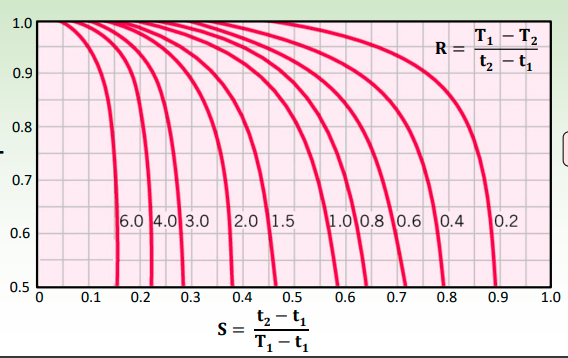
\includegraphics[width=0.8\textwidth]{R_S_Grafico}
\caption{Gráfico de \(R\) e \(S\) para o fator de correção \(F_{T}\)}
\label{fig:R_S_Grafico}
\end{figure}

A queda de pressão no lado da carcaça é dada por

\begin{equation}\label{eq:queda_pressao_carcaça}
    \frac{\Delta P_{\text{carcaça}}}{\rho } = f \frac{D_{c} \left( N+1 \right) }{D_{eq} }\frac{\upsilon ^{2} }{2}
\end{equation}
Onde é uma formula modificada da Lei de Darcy. \(N\) é o número de chicanas, \(D_{c}\) é o diâmetro 
da carcaça e \(D_{eq}\) é o diâmetro equivalente. \par

A queda de pressão no interior dos tubos é dada pela Lei de Darcy normal, ou seja:
\begin{equation}\label{eq:queda_pressao_tubo}
    \frac{\Delta P_{tubo}}{\rho } = f \frac{L_{eq} }{D_{eq} }\frac{\upsilon ^{2} }{2}
\end{equation}
Onde \(L_{eq}\) é o comprimento equivalente, que deve ser multiplicado pelo número de passagens.
\par
\subsection{Exemplo}
Numa industria há um trocador de calor tipo carcaça tubo 1:2 com 160 tubos de cobre BWG 18 de
\(\frac{3}{4}^{\prime \prime}\) e comprimento de 5 metros, arranjo triangular, pitch
\(\frac{15}{16}^{\prime \prime} \) com chicanas de espessura \(2.5 \;mm\) espaçadas de \(30 \; cm\).
Necessita-se saber se o trocador será adequado para resfriar \(80000 \; \frac{kg}{h}\) de água
destilada da temperatura de \(35 \; \degree C \to 30 \; \degree C\), dispondo de \(150000 \;
\frac{kg}{h}\) de água não tratada à \(22 \; \degree C\). A perda de carga admissível em cada
corrente é de 10 psi e o fator de incrustação é de \(0.0001 \) e \(0.0003 \; h m^{2} C / kcal\) para
água destilada e não tratada, respectivamente, desde que a velocidade não seja menor que 2 \(\frac{m}{s}\).       
 
\subsubsection{Solução}
Pelo método de Kern, vamos calcular a temperatura de saída do fluído frio. Pelo balanço de energia
temos
\begin{align}
    \dot{M}C_{p} \Delta T &= \dot{m}  c_p \Delta t \\
    t_2 &= t_1 + \frac{\dot{M} C_p \Delta T}{\dot{m}c_{p}}\\
    t_2 &= 22 + \frac{80000 \cdot 1 \cdot \left( 35 - 30 \right) }{150000 \cdot 1}\\
    t_2 &= 24.6667 \; \degree C
\end{align}
De acordo com nosso enunciado, as características do nosso trocador são:
\begin{itemize}
    \item {Carcaça:\\
            \begin{itemize}
            \item L = \(5 \; m\)  \\
            \item D = \(15 \frac{1}{4}^{\prime \prime} \)\\
            \item Passagem = 1\\
            \item Espessura Chicana = \(0.0025 \; m\) \\
            \item \(P_{T} \) = \(0.0238 \; m\) \\
            \item \(C^{\prime} \) = \(P_{T} - D_{e} = 0.00483 \; m\)\\
            \item B = \(0.3 \; m\) \\
            \end{itemize}
    }
    \item {Tubos:\\
            \begin{itemize}
            \item L = \(5 \; m\) \\
            \item \(D_{E}\)  = \(3/4^{\prime \prime} \)\\
            \item Passagem = 2\\
            \item \(D_{I}\) = \(0.0166 \; m\)\\
            \item Arranjo triangular\\
            \item N = 160\\  
            \end{itemize}
    }
\end{itemize}
Agora, vamos pegar as propriedades termofísicas, na temperatura média \(32.5 \; \degree C\) , da água destilada:
\begin{align}
    C_{p} &= 0.998 \; \frac{kJ}{kg \; ^{\circ}C} \\
    K &= 0.53 \; \frac{\mathcal{K} }{h m^{2} \degree C}\\
    \mu &= 0.798 \cdot 10^{-3} \; \frac{kg}{m \cdot s}\\
    \rho &= 995.6 \frac{kg}{m^{3}}
\end{align}
Para a água não tratada (\(23 \degree C\) ), temos:
\begin{align}
    C_{p} &= 0.998 \; \frac{kJ}{kg \; ^{\circ}C} \\
    K &= 0.51 \; \frac{\mathcal{K} }{h m^{2} \degree C}\\
    \mu &= 1 \cdot 10^{-3} \; \frac{kg}{m \cdot s}\\
    \rho &= 996.2 \frac{kg}{m^{3}}
\end{align}
Para calcular a \(MLDT\) temos de levar em conta que como são 2 passes, o primeiro será em
contra-corrente e o segundo em corrente paralela. Para as diferenças, temos \(\Delta T_1 = 35 - 24.7
= 10.3 \; \degree C\) e \(\Delta T_2 = 30 - 22 = 8 \degree C\). Portanto, nossa \(MLDT\) vale
\begin{align}
    MLDT &= \frac{\Delta T_1 - \Delta T_2}{\ln \frac{\Delta T_1}{\Delta T_2}}\\
    &= \frac{10.3 - 8}{\ln \frac{10.3}{8}}\\
    &= 9.1016 \; \degree C   
\end{align}
Agora, teremos que achar o valor verdadeiro de temperatura, primeiro vamos calcular \(S, R\)
\begin{align}
    R &= \frac{35 - 30}{24.7 - 22} = 1.8518 \\
    S &= \frac{24.7 - 22}{35 - 22} = 0.2077 \\
\end{align}
Com isso, vamos achar o fator de correção \(F_{T}\)
\begin{align}
    F_{T} &= \frac{\sqrt{R^{2} + 1} \ln \frac{1 - S}{1 - RS}}{\left( R -1 \right) \ln \frac{2 - S\left( R + 1 - \sqrt{R^{2} + 1}  \right) }{2 - S\left( R + 1 + \sqrt{R^{2} + 1}  \right) }}\\
    &= \frac{\sqrt{1.8518^{2} + 1} \ln \frac{1 - 0.2077}{1 - 1.8518 \cdot 0.2077}}{\left( 1.8518 -1 \right) \ln \frac{2 - 0.2077\left( 1.8518 + 1 - \sqrt{1.8518^{2} + 1}  \right) }{2 - 0.2077\left( 1.8518 + 1 + \sqrt{1.8518^{2} + 1}  \right) }}\\
    &= 0.9721
\end{align}
Ou, graficamente, que é bem mais fácil, chegaríamos num valor de \( \approx 0.97\). Com isso, nossa
temperatura real será
\begin{align}
    \Delta T_{real} &= 9.1016 \cdot 0.9721\\
    &= 8.8477 \; \degree C
\end{align}
Agora, vamos calcular o número de Reynolds para o lado da carcaça. Primeiro vamos precisar da área
de escoamento, que será
\begin{align}
    A_{escoamento, \text{carcaça}} &= \frac{P_{T} ^{2} \cdot 0.866}{2} - \frac{\pi D_{ext} ^{2} }{2 \cdot 4}\\
    &= \frac{0.0238^{2} \cdot 0.866}{2} - \frac{\pi \cdot 0.0191^{2} }{2 \cdot 4}\\
    &= 1.0201 \cdot 10^{-4} \; m^{2}
\end{align}
O perímetro molhado é dado por
\begin{align}
    P_{m} &= \pi \frac{D_{ext}}{2}\\
    &= \pi \frac{0.0191}{2}\\
    &= 0.03 \; m
\end{align}
Agora, nosso diâmetro equivalente é dado por
\begin{align}
    D_{eq} &= \frac{4 \cdot A_{escoamento, \text{carcaça}}}{P_{m} \cdot N}\\
    &= \frac{4 \cdot 1.0201 \cdot 10^{-4}}{0.03 \cdot 160}\\
    &= 8.501 \cdot 10^{-5}
\end{align}
Agora, vamos calcular a área superficial
\begin{align}
    A_{escoamento, \text{carcaça}} &= \frac{D_{I} c^{\prime} B}{P_{T} } \\
    A_{escoamento, \text{carcaça}} &= \frac{0.387 \cdot 0.00483 \cdot 0.3}{0.0238}\\
    &= 0.02356 \; m^{2} 
\end{align}

Agora vamos calcular a velocidade

\begin{align}
    \upsilon &= \frac{\dot{m}}{\rho A_{escoamento, \text{carcaça}}}\\
    &= \frac{80000 \cdot 1/3600}{995.6 \cdot 0.02356}\\
    &= 0.9474 \; \frac{m}{s}
\end{align}
O número de Reynolds é dado por
\begin{align}
    Re &= \frac{\rho \upsilon D_{eq} }{\mu }\\
    &= \frac{995.6 \cdot 0.9474 \cdot 8.501 \cdot 10^{-5}}{0.798 \cdot 10^{-3}}\\
    &= 100.4813
\end{align}
O regime é laminar. Vamos calcular o número de Reynolds para o lado dos tubos. Primeiro, vamos
calcular a velocidade
\begin{align}
    \upsilon &= \frac{\dot{m}}{\rho A_{escoamento, tubo}}\\
    &= \frac{150000 \cdot 1/3600}{996.2 \cdot \frac{\pi \cdot 0.0166^{2} \cdot 160}{4 \cdot 2}}\\
    &= 2.4157 \; \frac{m}{s}
\end{align}
O número de Reynolds é dado por
\begin{align}
    Re &= \frac{\rho \upsilon D_{eq} }{\mu }\\
    &= \frac{996.2 \cdot 2.4157 \cdot 0.0166}{1 \cdot 10^{-3}}\\
    &= 39948.2376
\end{align}
Sendo turbulento. Vamos calcular o número de Proust para o lado tubo:
\begin{align}
    Pr &= \frac{C_{p} \mu}{K}\\
    &= \frac{0.998 \cdot 1 \cdot 10^{-3} \cdot 3600}{0.51}\\
    &= 7.0447
\end{align}
Agora, para o lado carcaça
\begin{align}
    Pr &= \frac{C_{p} \mu}{K}\\
    &= \frac{0.998 \cdot 0.798 \cdot 10^{-3} \cdot 3600}{0.53}\\
    &= 5.4095
\end{align}
Agora, vamos calcular o número de Nusselt para o lado dos tubos
\begin{align}
    Nu &= \frac{hD}{K} = 0.023 \left[ 1 + \left( \frac{D}{L} \right) ^{0.7}  \right] Re^{0.8} Pr^{0.33} \left( \frac{\mu _{b} }{\mu _{p} } \right) ^{0.14}\\
    &= 0.023 \left[ 1 + \left( \frac{0.0166}{5} \right) ^{0.7}  \right] 39948.2376^{0.8} 7.0447^{0.33} \left( \frac{1 \cdot 10^{-3}}{1 \cdot 10^{-3}} \right) ^{0.14}\\
    &= 214.11079 
\end{align}
O coeficiente de transferência de calor é dado por
\begin{align}
    h &= \frac{Nu K}{D}\\
    &= \frac{214.11079 \cdot 0.51}{0.0166}\\
    &= 6578.10258 \; \frac{kcal}{h \cdot m^{2} \; ^{\circ}C}
\end{align}
Agora, vamos calcular o número de Nusselt para o lado da carcaça
\begin{align}
    Nu &= 0.36 \left( \frac{D_{eq} \rho \upsilon }{\mu } \right)^{0.55} \left( \frac{\mu c_{p} }{k} \right)^{\frac{1}{3}} \left( \frac{\mu }{\mu _{p} } \right) ^{0.14}\\
    &= 0.36 \left(\frac{8.501 \cdot 10^{-5} \cdot 995.6 \cdot 0.9474 }{0.798 \cdot 10^{-3}}  \right)^{0.55} \left( \frac{0.798 \cdot 10^{-3} \cdot 4180 }{0.53} \right)^{\frac{1}{3}} \left( \frac{0.798 \cdot 10^{-3} }{0.798 \cdot 10^{-3}} \right) ^{0.14}\\
    &= 8.3898 
\end{align}
%To do, arrumar essa conta
O coeficiente de transferência de calor é dado por
\begin{align}
    h &= \frac{Nu K}{D_{eq}}\\
    &= \frac{8.3898 \cdot 0.53}{8.501 \cdot 10^{-5}}\\
    &= 52306.71686 \; \frac{kcal}{h \cdot m^{2} \; ^{\circ}C}
\end{align}
Vamos determinar o coeficiente global de transferência de calor
\begin{align}
    U_{sujo} &= \left( \frac{1}{h_{i} }\frac{D_E}{D_{i} } + \frac{D_E}{2K} \ln \frac{D_E}{D_{i} } + \frac{1}{he} + R_{di} + R_{dE}  \right)^{-1} \\
    &= \left( \frac{1}{6578.10258} \cdot  \frac{0.0191}{0.0166} + \frac{0.0191}{2 \cdot 342.3} \cdot  \ln \left( \frac{0.0191}{0.0166} \right)  + \frac{1}{52306.71686} + 0.0001 + 0.0003  \right)^{-1}\\
    &= 1672.3920 \; \frac{kcal}{h m^{2} \degree C}\\
\end{align}
A área de troca de calor é dada por
\begin{align}
    A_{t} &= \frac{Q}{U_{sujo} MLDT}\\
    &= \frac{80000 \cdot 1 \cdot \left( 35 - 30 \right) }{1672.3920 \cdot 9.1016}\\
    &= 26.2787 \; m^{2}
\end{align} 
Falta agora descobrir as perdas de carga. Primeiro, vamos calcular para os tubos. Como o tubo é
liso, seu fator de atrito vale \(0.022\). Vamos utilizar a formula de Darcy-Weisbach
\begin{align}
    \frac{\Delta P}{\rho } &= \frac{fL_{eq} }{D} \frac{\upsilon ^{2}}{2}\\
    &= 0.022 \frac{2 \cdot 5}{0.0166} \frac{2.4157^{2}}{2}\\
    &= 38.6697 \; \frac{J}{kg}
\end{align}
Agora, vamos calcular a perda de carga no retorno
\begin{align}
    \left(\frac{\Delta P}{\rho }\right)_{retorno} &= 4 \cdot \left( \frac{\upsilon ^{2}}{2}  \right) \rho \\
    &= 4 \cdot \left( \frac{2.4157^{2}}{2}  \right)\\
    &= 11.6712 \; \frac{m^{2} }{s ^{2} }
\end{align}
A perda total nos tubos é a soma das duas, logo
\begin{align}
    \left(\frac{\Delta P}{\rho }\right)_{tubo} &= 38.6697 + 11.6712\\
    &= 50.3409 \; \frac{m^{2} }{s ^{2} } \cdot 996.2 \frac{kg}{m  ^{3}} \cdot \frac{1.45 \cdot 10^{-4}}{1 \text{pascal}}\\
    &= 7.2716926641 \; psi
\end{align}
Agora, vamos calcular a perda de carga na carcaça. Como o regime é laminar, nosso fator de atrito é
achado pelo gráfico de Moody, que vale \(f = 0.864\). Através da formula de Darcy-Weisbach,
modificada, \eqref{eq:queda_pressao_carcaça}, temos
\begin{align}
    \frac{\Delta P}{\rho } &= f \frac{D_{c} \left( N+1 \right) }{D_{eq} }\frac{\upsilon ^{2} }{2}\\
    &= 0.864 \frac{0.387 \cdot \left( 16 + 1 \right) }{8.501 \cdot 10^{-5}} \frac{0.9474^{2}}{2}\\
    &= 30008.2299 \; \frac{m^{2} }{s ^{2} } \cdot 995.6 \frac{kg}{m  ^{3}} \cdot \frac{1.45 \cdot 10^{-4}}{1 \text{pascal}}\\
    &= 4332.0480848238 \; psi
\end{align}
%Acho que isso ta resolvido
